In recent years the rise of Big Data, large volumes of various structured and unstructured data types at a high velocity, has showed an incredible potential but it has also posed a number of challenges \cite{penceWhatBigData2014}. These mostly impact the software architecture that needs to deal with these issues, that lead to an evolution of these technologies \cite{gortonDistributionDataDeployment2015}. Delta Lake \cite{armbrustDeltaLakeHighperformance2020}, is one of the most recent iteration of this evolution process, but in order to understand the tool, it is necessary to understand the challenges, starting from the beginning of the data management evolution.

Before Big Data, companies already wanted to gain insights from their data sources using an automated workflow. Here is where \gls{ETL} and relational databases first came in use. An \gls{ETL} pipeline as the name suggests:
\begin{enumerate}
    \item Extracts data from \glspl{API} or other company's data sources.
    \item Transforms data by removing errors or absent fields, standardises the format to match the database and validate the data to verify its correctness.
    \item Loads it into a relational database (e.g. MySQL).
\end{enumerate} 

\begin{figure}[!ht]
    \begin{center}
      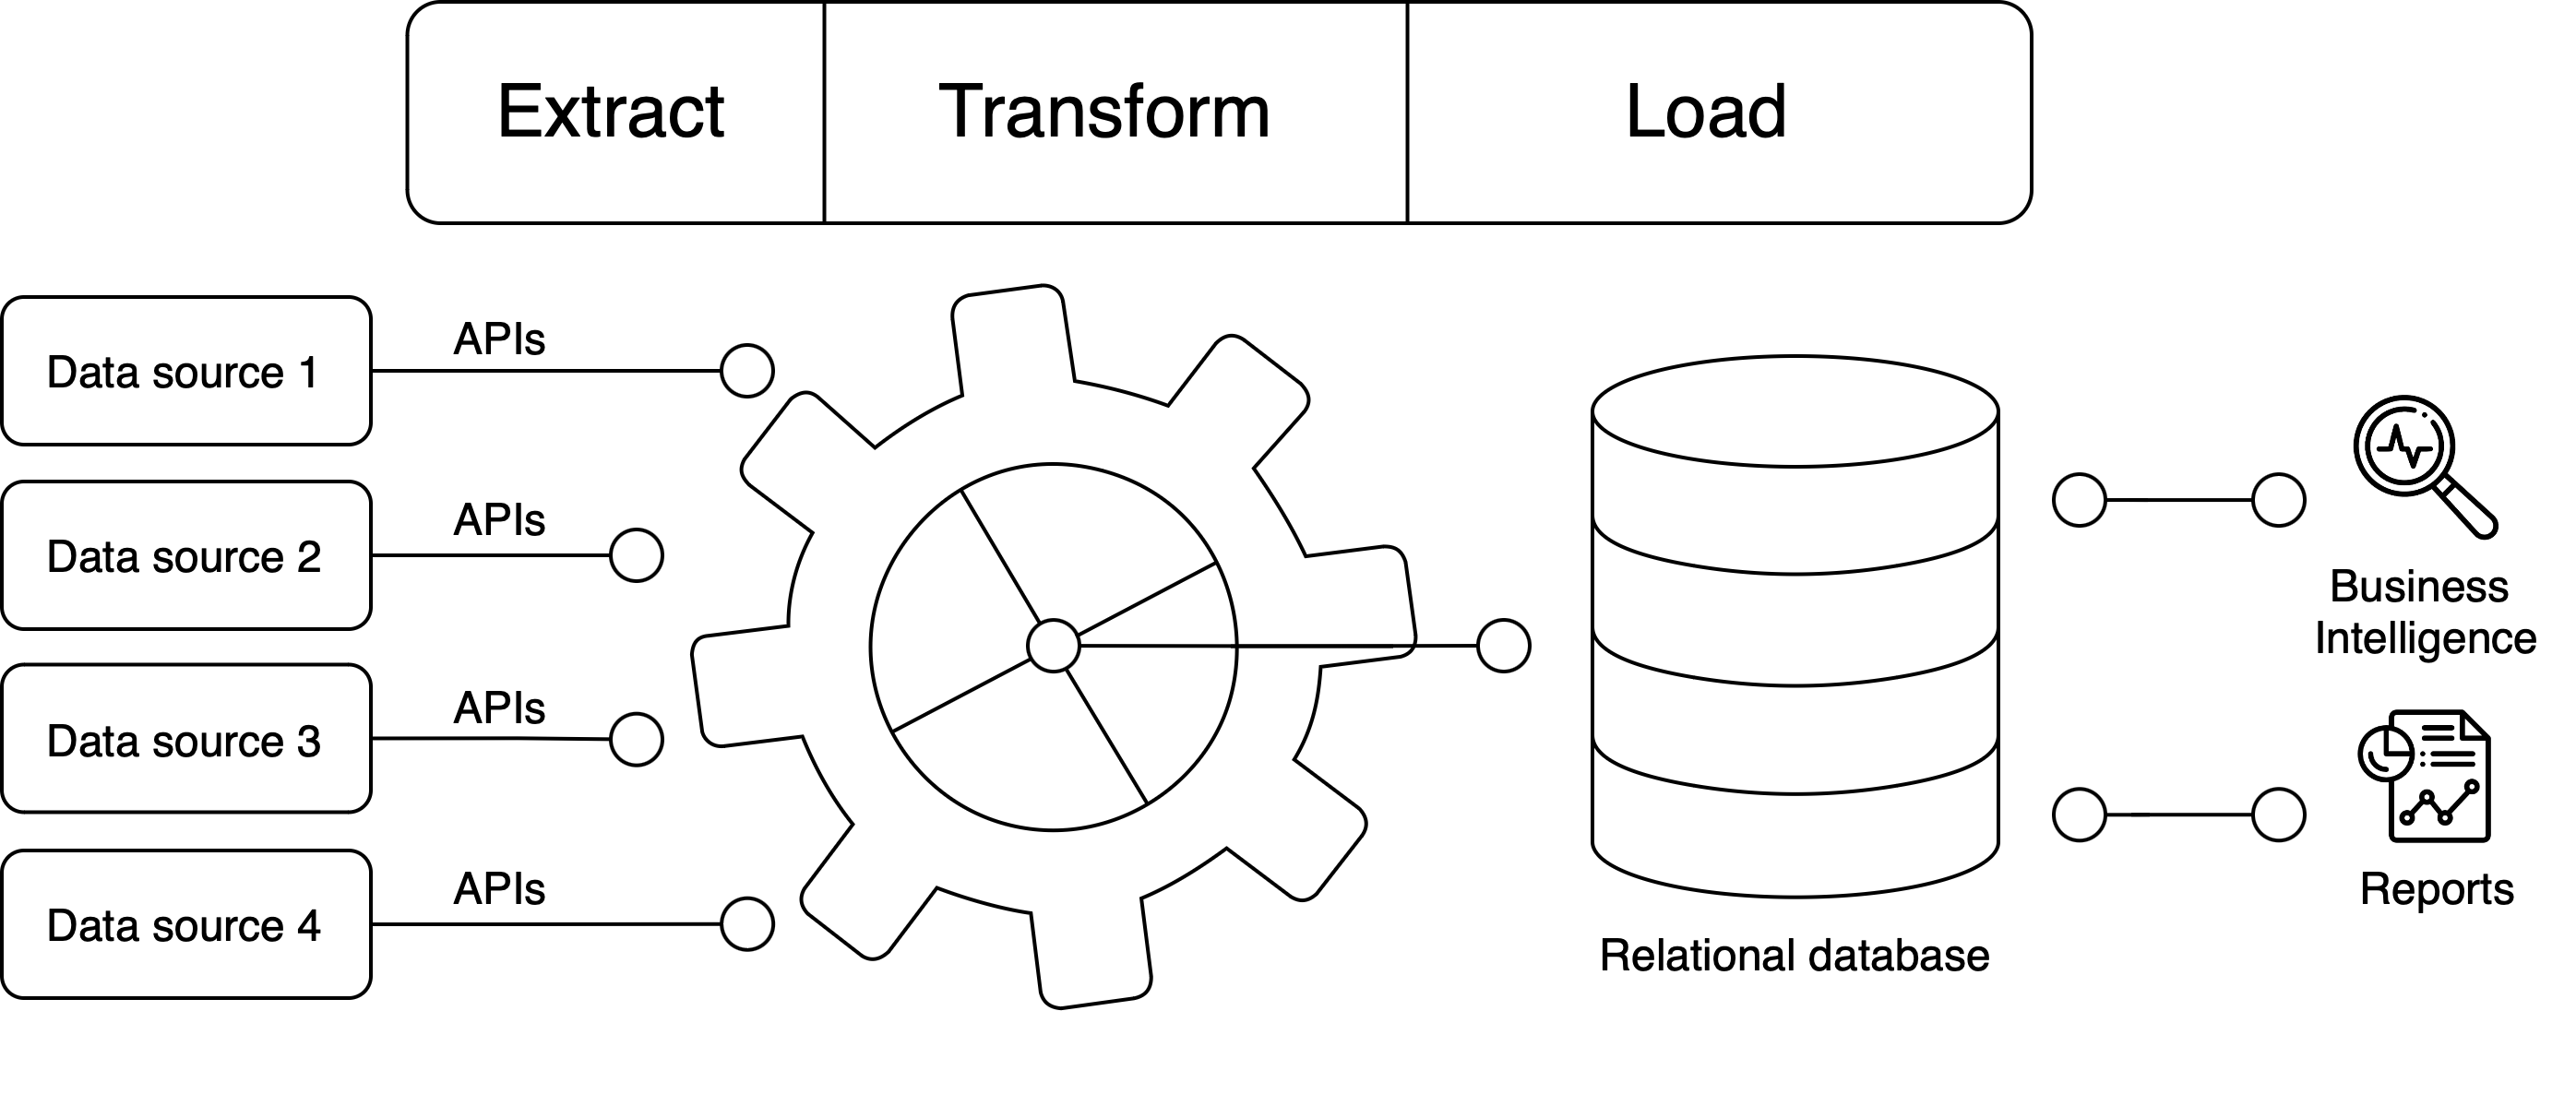
\includegraphics[width=\textwidth]{figures/2-background/DeltaLake_evolution-ETL+DB.png}
    \end{center}
    \caption{Simple \gls{ETL} system with a relational database. Figure inspired by AltexSoft video \cite{altexsoftHowDataEngineering2021}}
    \label{fig:ETL+DB}
\end{figure}

This type of workflow worked for companies with no need of running complex analytical queries. This type of relational databases focusing on transactions are called \gls{OLTP} in contrast to \gls{OLAP} systems. When the need to compute more complex queries rose, \gls{DBMS} substituted simple database tables, optimized for running business centric complex analytical queries.

\begin{figure}[!ht]
    \begin{center}
      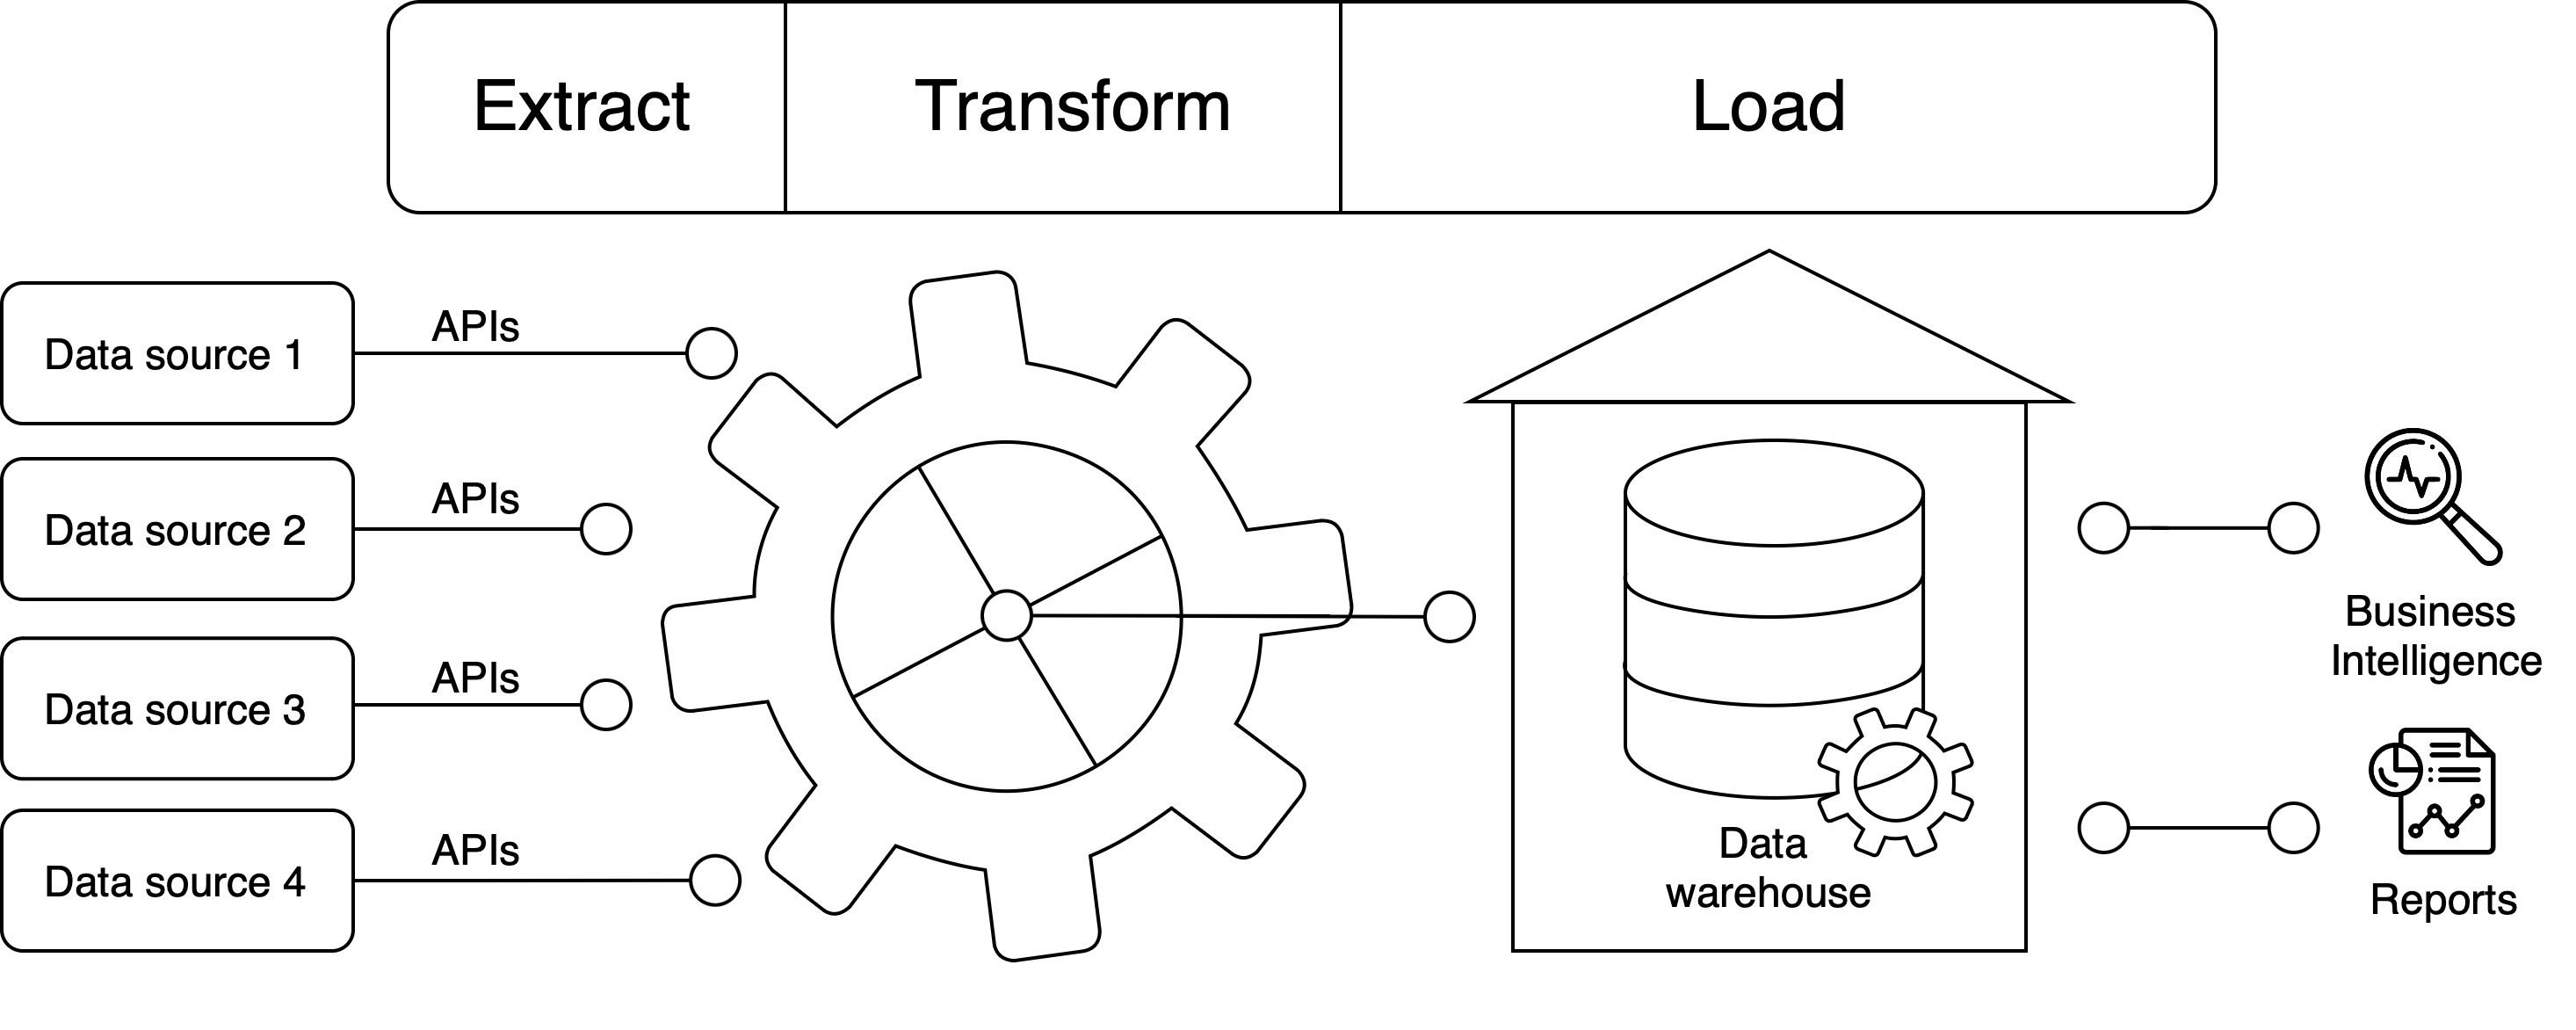
\includegraphics[width=\textwidth]{figures/2-background/DeltaLake_evolution-ETL+DW.png}
    \end{center}
    \caption{\gls{ETL} system with a data warehouse. Figure inspired by AltexSoft video \cite{altexsoftHowDataEngineering2021}}
    \label{fig:ETL+DW}
\end{figure}

Here is where the first challenges caused by Big Data rose. \gls{DBMS} only support structured data, while Big Data can be unstructured (e.g. images, videos). Furthermore, storing large \gls{DBMS} systems is expensive and does not support any type of \gls{AI}/\gls{ML} workflow.

These issues were tackled by a new paradigm called Data Lake. Data Lakes are based on a low cost object storage system (see \ref{sec:dis_storage} to know more) that consist of a flat structure where all data is loaded after extraction. In Data lakes we have \gls{ELT} pipelines that leave transformation customizable for specific applications. This architecture reduces storage costs, but the increase in complexity might make the architecture ultimately cost more depending on the case. 

\todo[inline]{Explain the higher complexity of the new structure}

\begin{figure}[!ht]
    \begin{center}
      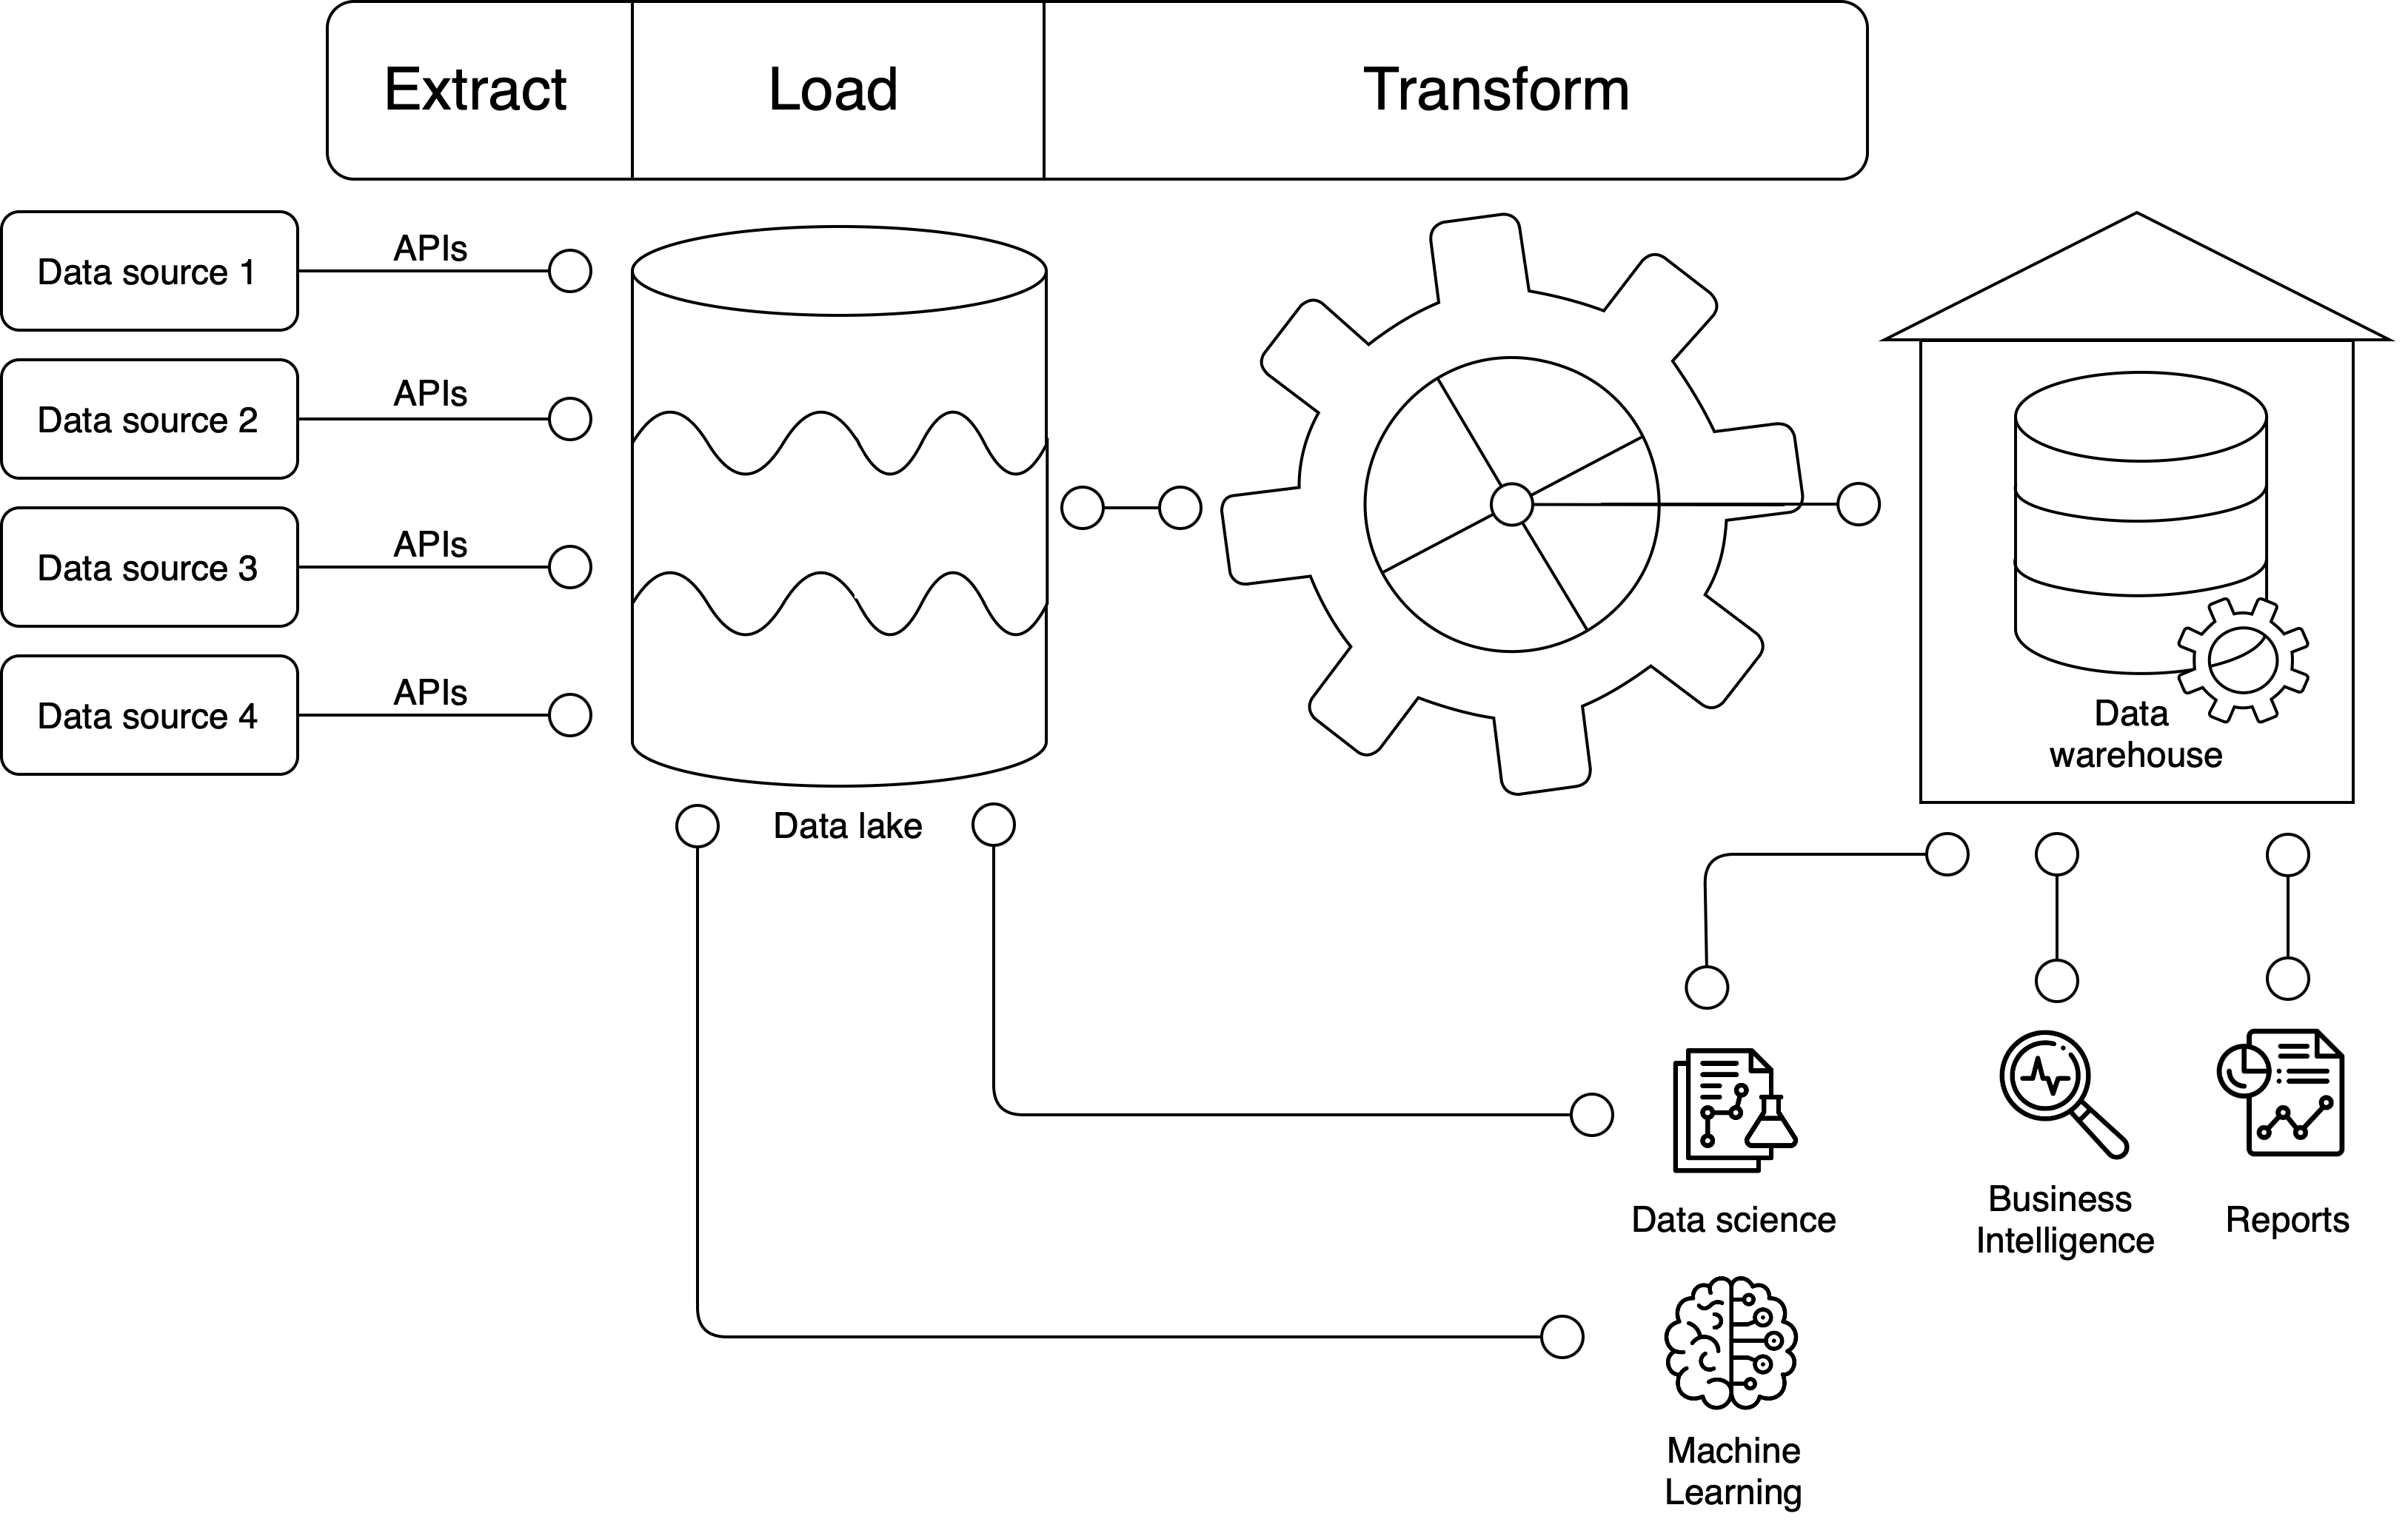
\includegraphics[width=\textwidth]{figures/2-background/DeltaLake_evolution-ELT+DL.png}
    \end{center}
    \caption{\gls{ELT} system with a data lake. Figure inspired by AltexSoft video \cite{altexsoftHowDataEngineering2021}}
    \label{fig:ETL+DL}
\end{figure}